\documentclass[11pt,a4paper]{article}
\usepackage[left=1in,right=1in,top=19mm,bottom=24mm,footskip=11mm]{geometry}
\usepackage[T1]{fontenc}
\usepackage{lmodern,amsmath,amssymb,graphicx,booktabs,longtable,array,url}
\usepackage[hidelinks]{hyperref}
\frenchspacing\raggedbottom\setlength{\parindent}{0pt}\emergencystretch=2em
\newcommand{\routetitle}[3]{\noindent{\Large\bfseries #1\quad #2}\hfill{\small #3}\par\vspace{1mm}\hrule\vspace{0mm}}
\newcommand{\figcap}[1]{\par\smallskip{\centering\begin{minipage}{.94\textwidth}\small\centering #1\end{minipage}\par}}
\begin{document}

\thispagestyle{empty}\setcounter{page}{0}
\noindent{\LARGE\bfseries An atlas of proof routes for Barnette\textquotesingle s conjecture}\par\medskip
\noindent Readings of one proof, each drawn on a computed example. The proof is the one in the OpenAI paper: every cubic, bipartite, 3-connected planar graph $G$ has a Hamiltonian cycle. Most pages use one triangulation $T$ with 13 vertices, the dual of a graph $G$ with 22 vertices. Black faces of $T$ are grey, the outer black face is the grey collar, and the three roots are hollow. A state is a set of filled corner wedges, one in each black face. Page 1 is the map. The last page lists where each picture and number comes from.\par\vfill
\noindent\begin{tabular}{@{}c@{\hspace{2.9mm}}c@{\hspace{2.9mm}}c@{\hspace{2.9mm}}c@{\hspace{2.9mm}}c@{}}
\begin{minipage}[t]{2.95cm}\centering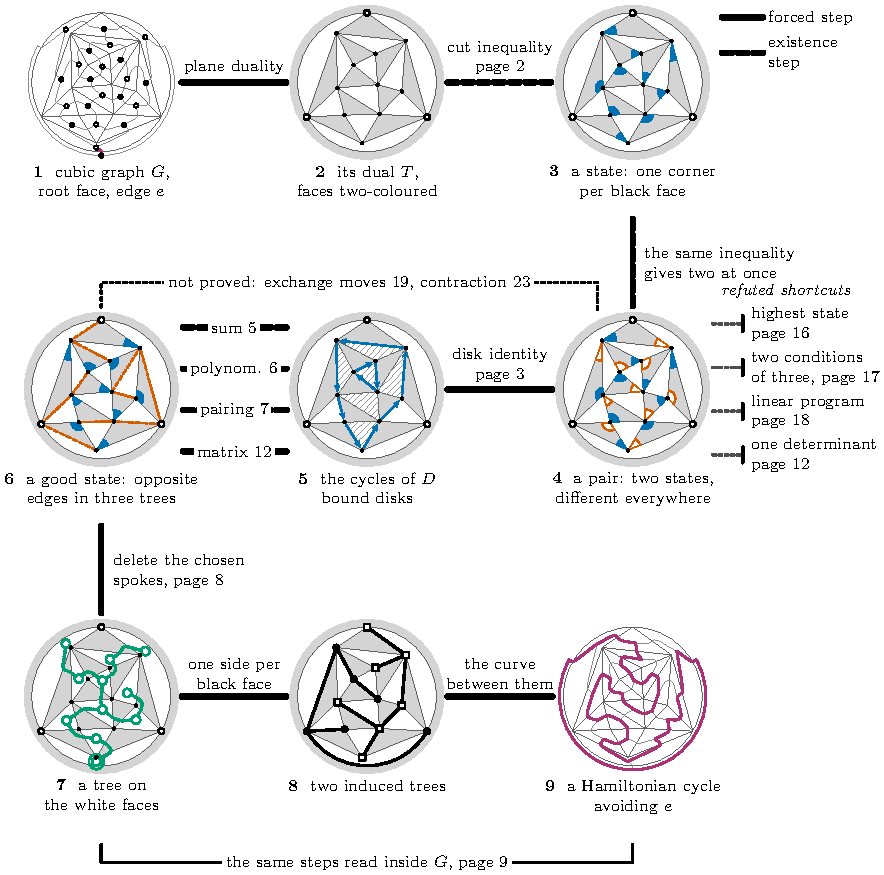
\includegraphics[width=2.75cm,height=2.35cm,keepaspectratio]{figs/01-chain.pdf}\\[.3mm]\footnotesize\raggedright\hyperlink{r1}{\textbf{1}\ The chain}\end{minipage} & \begin{minipage}[t]{2.95cm}\centering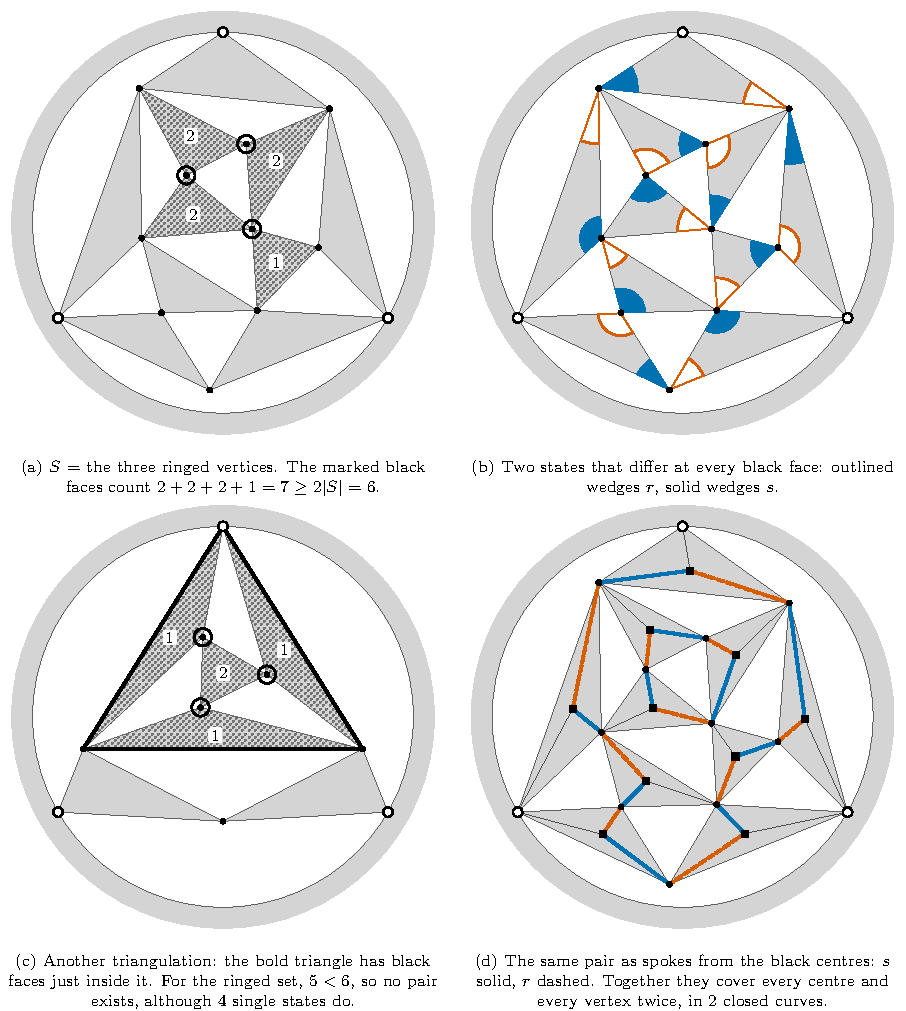
\includegraphics[width=2.75cm,height=2.35cm,keepaspectratio]{figs/02-pairs.pdf}\\[.3mm]\footnotesize\raggedright\hyperlink{r2}{\textbf{2}\ Two states}\end{minipage} & \begin{minipage}[t]{2.95cm}\centering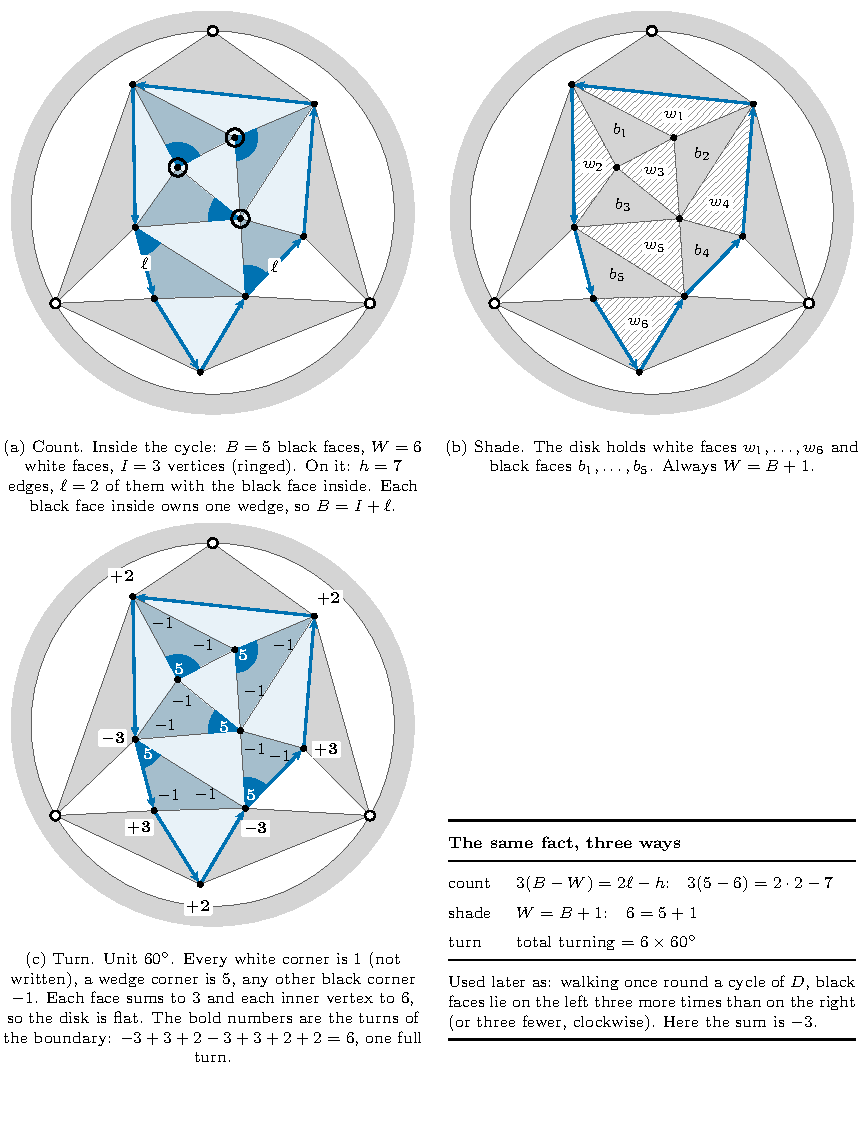
\includegraphics[width=2.75cm,height=2.35cm,keepaspectratio]{figs/03-disk.pdf}\\[.3mm]\footnotesize\raggedright\hyperlink{r3}{\textbf{3}\ Disk identity}\end{minipage} & \begin{minipage}[t]{2.95cm}\centering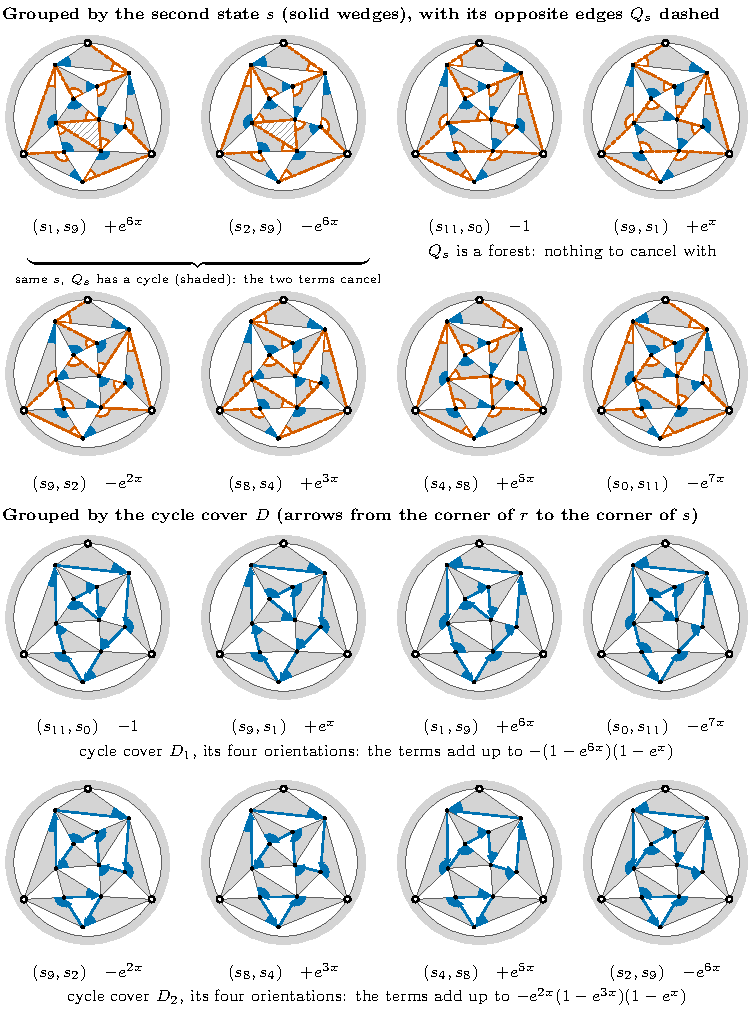
\includegraphics[width=2.75cm,height=2.35cm,keepaspectratio]{figs/04-sum.pdf}\\[.3mm]\footnotesize\raggedright\hyperlink{r4}{\textbf{4}\ Exponential sum}\end{minipage} & \begin{minipage}[t]{2.95cm}\centering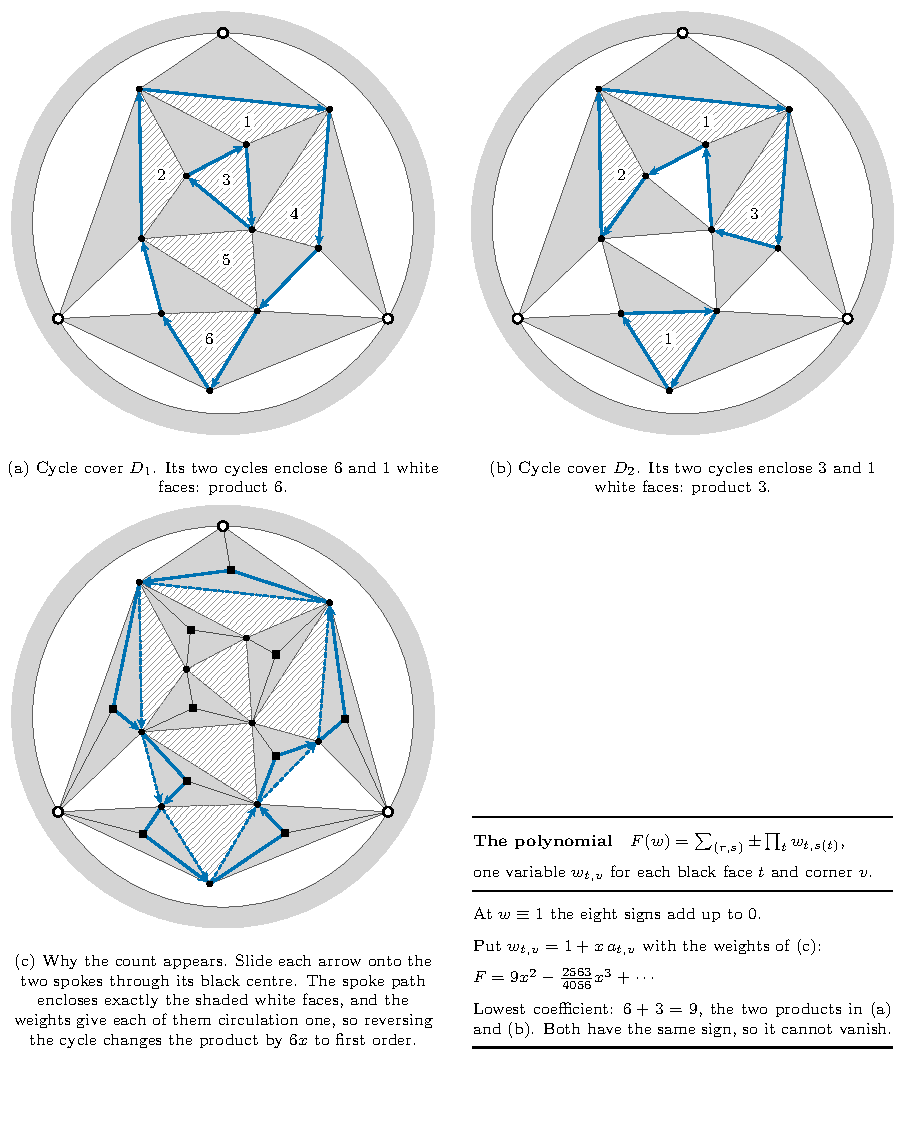
\includegraphics[width=2.75cm,height=2.35cm,keepaspectratio]{figs/05-polynomial.pdf}\\[.3mm]\footnotesize\raggedright\hyperlink{r5}{\textbf{5}\ Integer polynomial}\end{minipage}\\[2.2mm]
\begin{minipage}[t]{2.95cm}\centering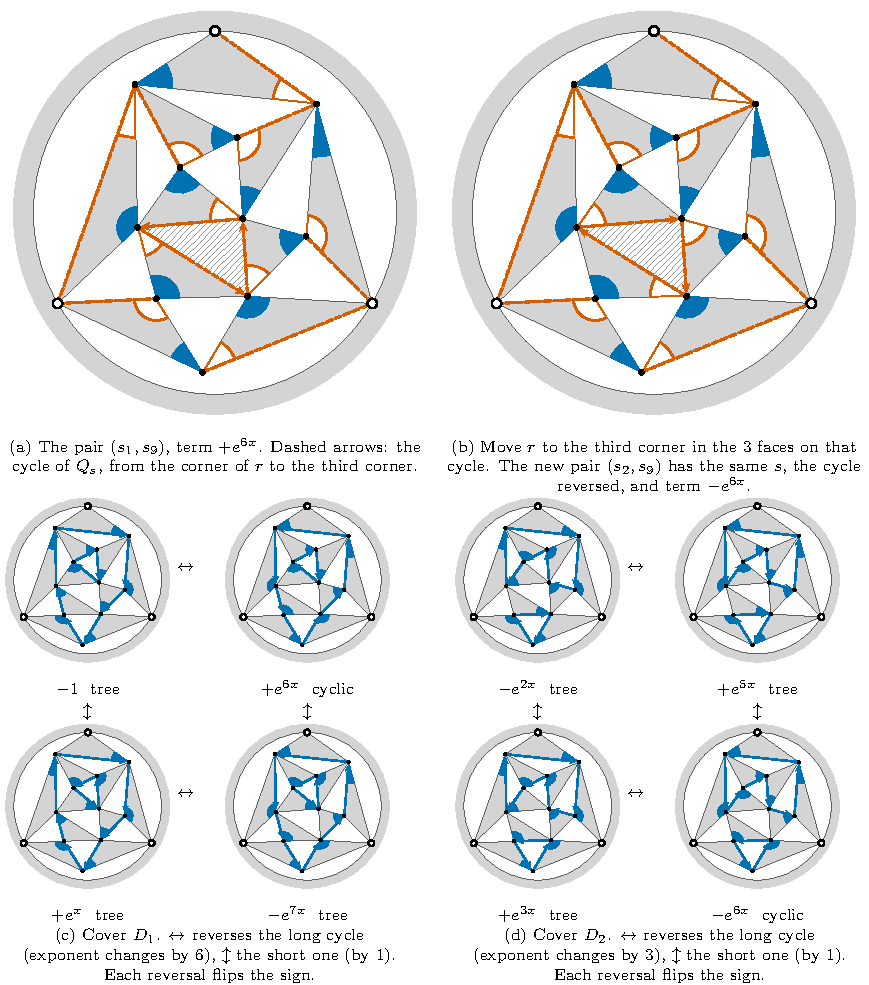
\includegraphics[width=2.75cm,height=2.35cm,keepaspectratio]{figs/06-involutions.pdf}\\[.3mm]\footnotesize\raggedright\hyperlink{r6}{\textbf{6}\ Involutions}\end{minipage} & \begin{minipage}[t]{2.95cm}\centering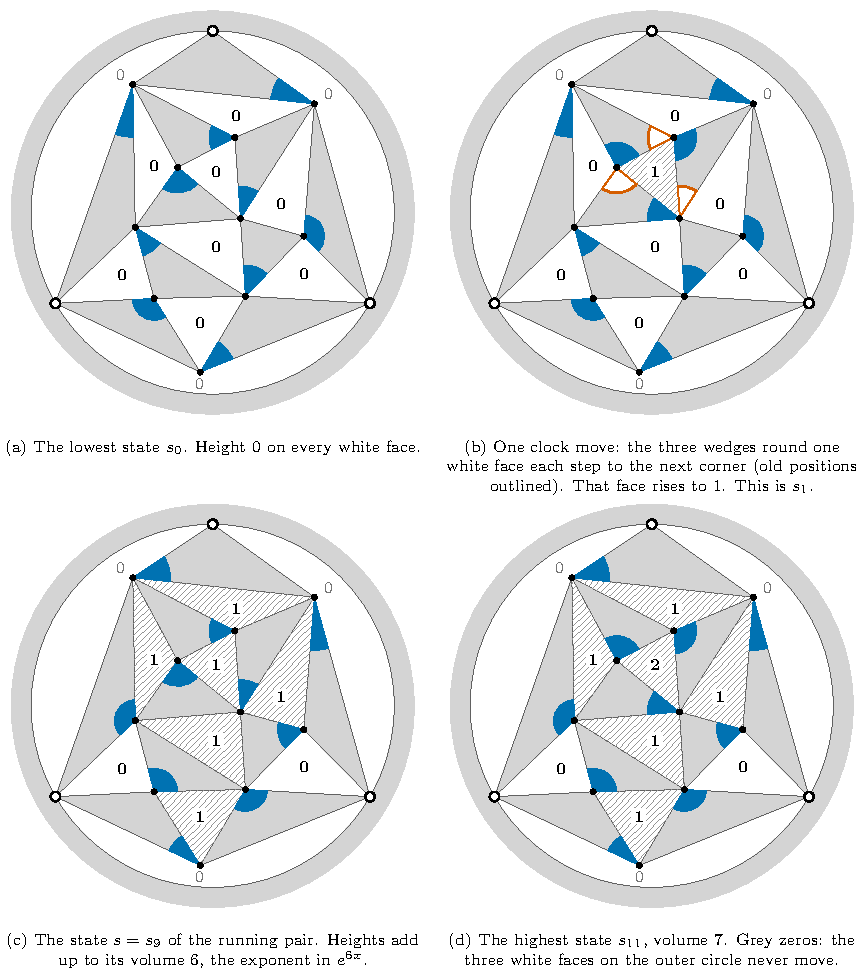
\includegraphics[width=2.75cm,height=2.35cm,keepaspectratio]{figs/07-heights.pdf}\\[.3mm]\footnotesize\raggedright\hyperlink{r7}{\textbf{7}\ Heights}\end{minipage} & \begin{minipage}[t]{2.95cm}\centering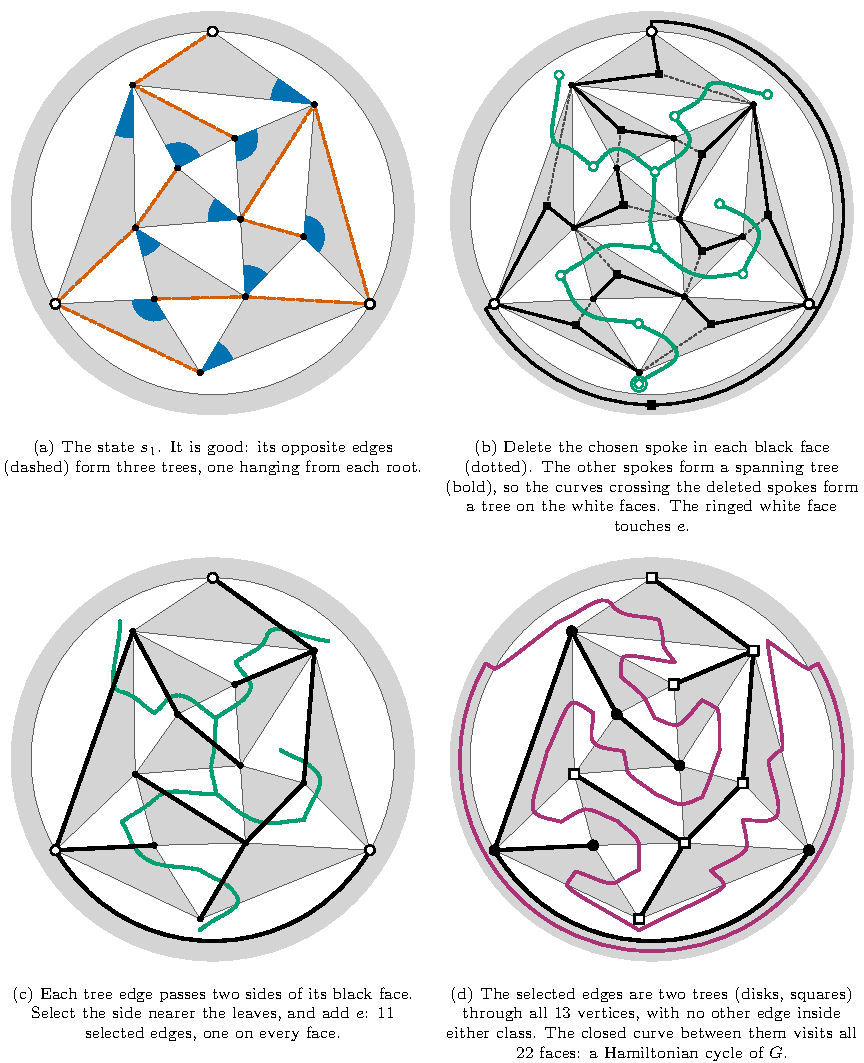
\includegraphics[width=2.75cm,height=2.35cm,keepaspectratio]{figs/08-recovery.pdf}\\[.3mm]\footnotesize\raggedright\hyperlink{r8}{\textbf{8}\ Recovery}\end{minipage} & \begin{minipage}[t]{2.95cm}\centering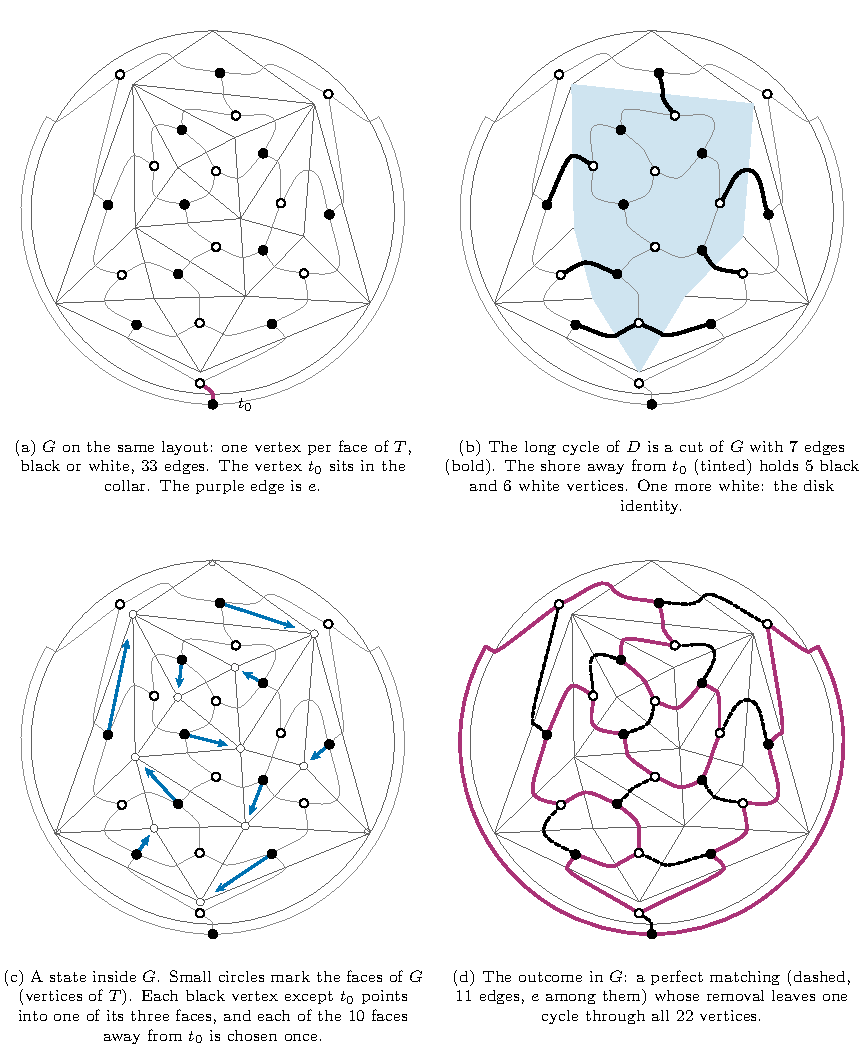
\includegraphics[width=2.75cm,height=2.35cm,keepaspectratio]{figs/09-primal.pdf}\\[.3mm]\footnotesize\raggedright\hyperlink{r9}{\textbf{9}\ Primal picture}\end{minipage}
\end{tabular}\par\vfill
\clearpage\hypertarget{r1}{}\routetitle{1}{The chain, and where the routes branch}{main chain}
\vfill{\centering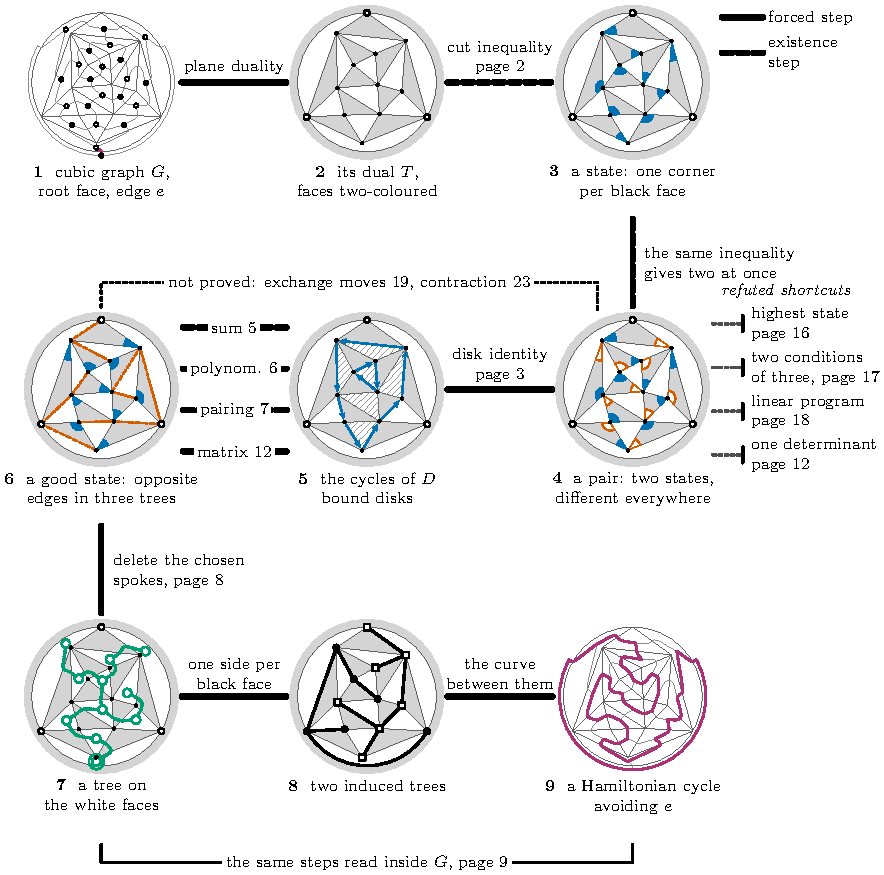
\includegraphics{figs/01-chain.pdf}\par}
\vfill\vfill Read the stations in order. The proof turns a cubic graph into its dual triangulation, finds two states that disagree at every black face, and shows that some state has a forest of opposite edges. From such a state, three constructions with no choices in them build the Hamiltonian cycle. Only the step from station 5 to station 6 is hard, and the atlas has four readings of it. They are four ways to organise one argument, a signed sum that cancels the cyclic states and still cannot vanish. They are not four proofs. The stubs are shortcuts that this project tested and refuted with explicit examples. The dotted line marks two routes that would avoid the sum. Neither is proved.\par\smallskip \textbf{Status.} The chain is the proof in the OpenAI paper, Sections 3 to 7. Every thumbnail is computed on the running example.\par\vfill
{\small\textbf{See also}\quad 2 (two states), 3 (disk identity), 4 (exponential sum), 8 (recovery).\par}
\clearpage\hypertarget{r2}{}\routetitle{2}{Two states from one count}{main chain}
\vfill{\centering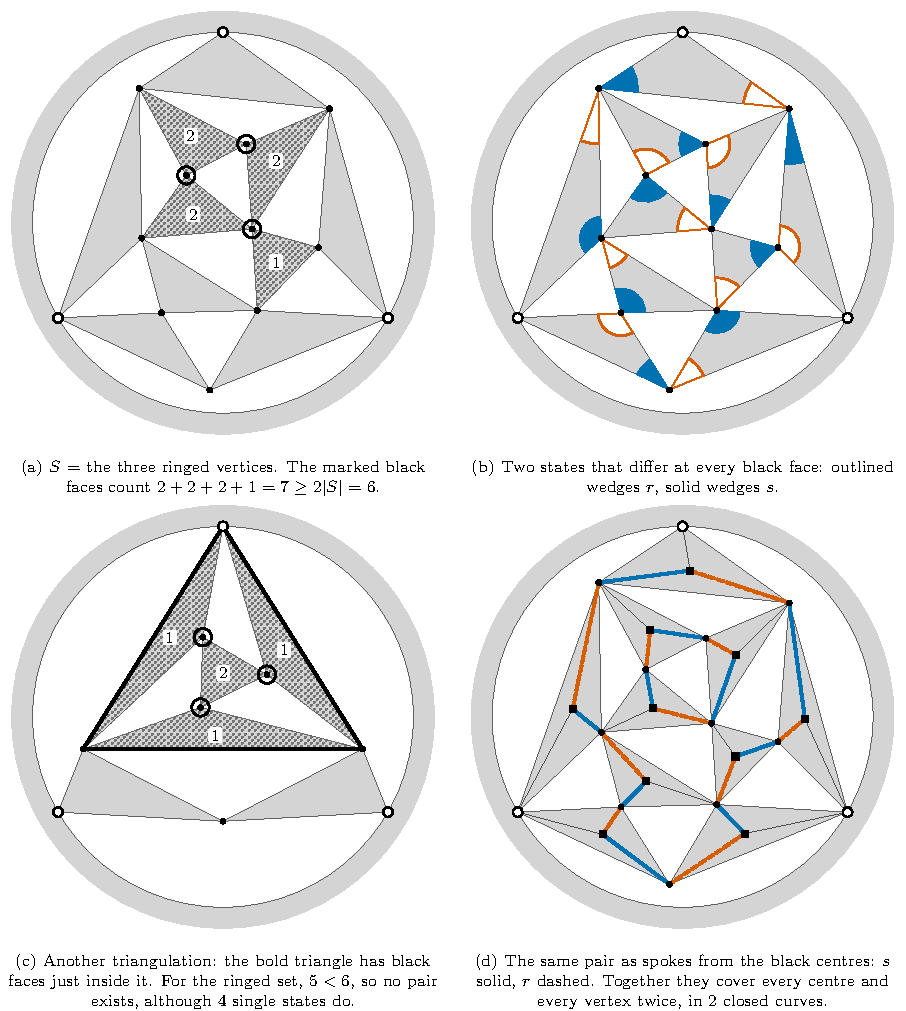
\includegraphics{figs/02-pairs.pdf}\par}
\vfill\vfill A state gives each bounded black face one of its corners, uses no root, and uses every other vertex once. The proof needs two states that disagree at every face. A doubled form of Hall's theorem says they exist when every set $S$ of non-root vertices passes one count. Each black face scores the number of its corners in $S$, capped at two, and the scores must add up to at least $2|S|$. The count can fail. In (c) a separating triangle has black faces just inside it, the three vertices inside score five against a required six, and no pair exists. The paper cuts along separating triangles first, so that the count passes on every piece.\par\smallskip \textbf{Status.} OpenAI paper, Proposition 3.1 and Section 7. The checker tests all 1024 sets $S$ on the running example and the failing set in (c).\par\vfill
{\small\textbf{See also}\quad 1 (the chain).\par}
\clearpage\hypertarget{r3}{}\routetitle{3}{The disk identity, three ways}{main chain}
\vfill{\centering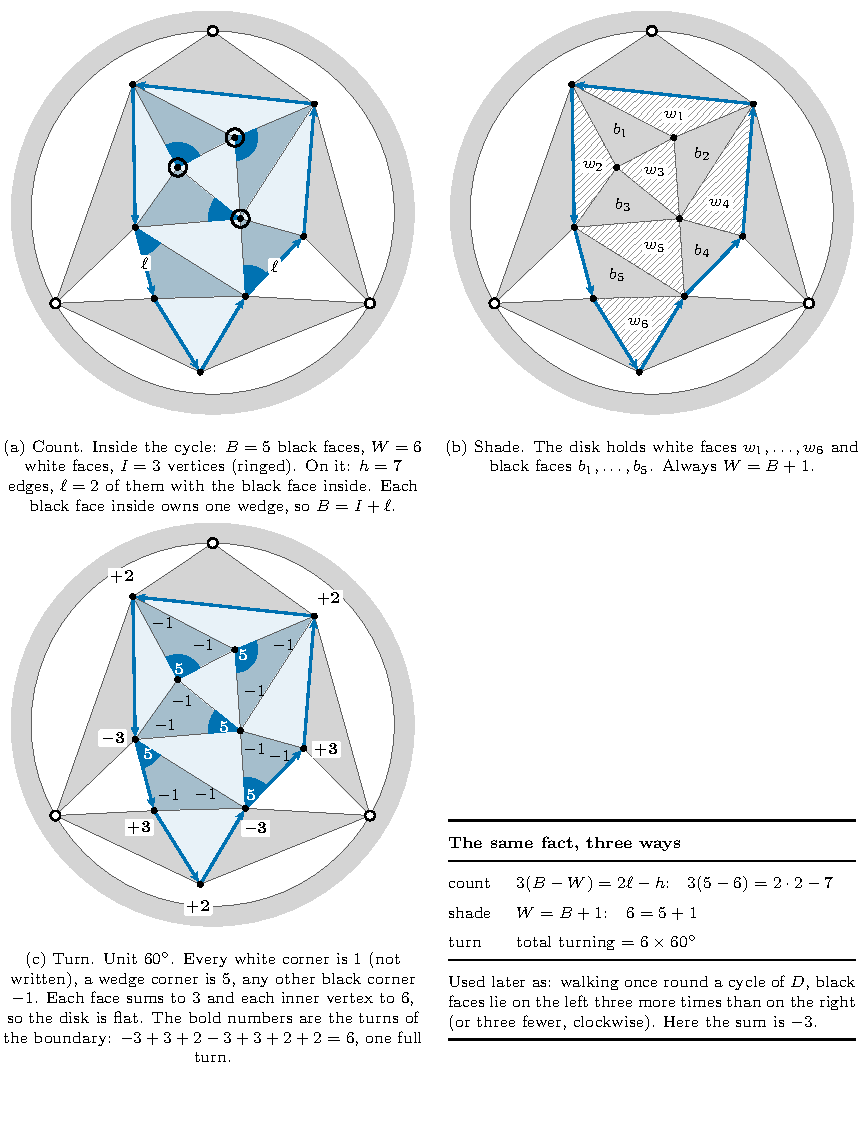
\includegraphics{figs/03-disk.pdf}\par}
\vfill\vfill Take a cycle of $D$ and the disk it bounds on the side away from the root face. Three arguments reach the same fact about that disk. Euler's formula, with one wedge for each black face inside, gives $3(B-W)=2\ell-h$. Shading shows one more white face than black. Reading corners as angles makes the disk flat, so its boundary turns exactly once. Each version says the same thing about a walk around the cycle. Black faces lie on the left three more times than on the right, or three fewer if the walk is clockwise. That fixed number is why the signs on page 4 behave.\par\smallskip \textbf{Status.} Lemma 4.1 of the OpenAI paper. The shading and turning versions were proved in this project and checked by a second model. No human has read them.\par\vfill
{\small\textbf{See also}\quad 4 (exponential sum), 5 (integer polynomial), 9 (primal picture).\par}
\clearpage\hypertarget{r4}{}\routetitle{4}{Eight terms, grouped twice}{main chain}
\vfill{\centering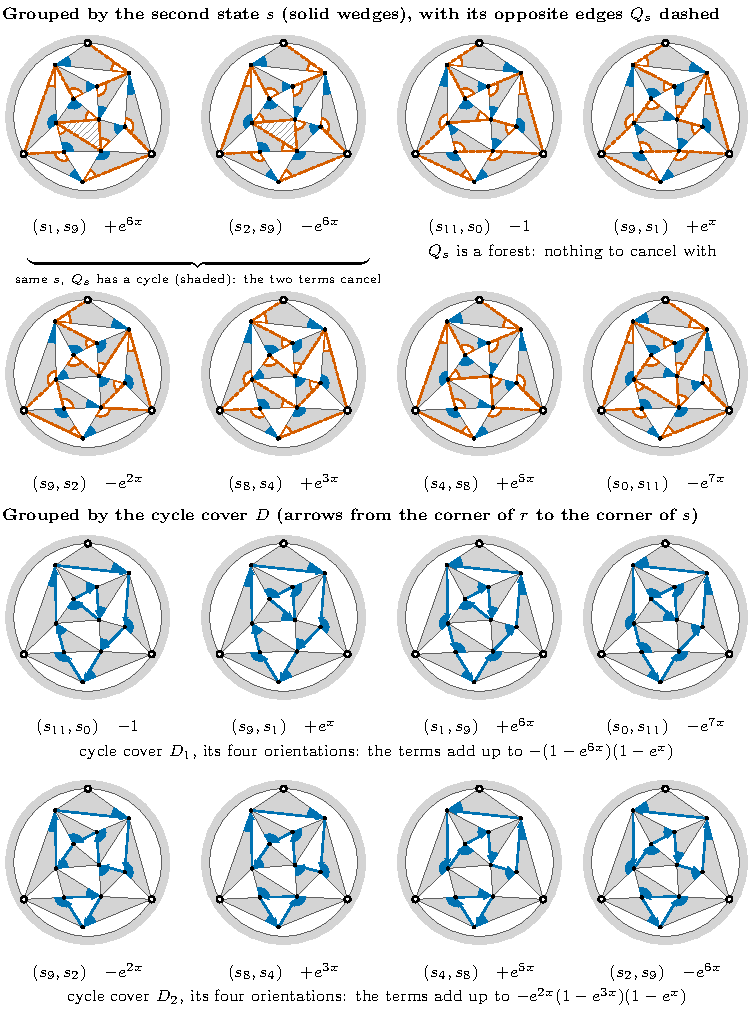
\includegraphics{figs/04-sum.pdf}\par}
\vfill\vfill Give every state $s$ an exponent, its volume from page 7, and every pair $(r,s)$ a sign read off the cycles of $D$. The eight pairs of the running example give eight terms $\pm e^{vx}$. Group them by $s$. The two pairs that share a cyclic $Q_s$ cancel, so only states with a forest survive. Group the same terms by the cycle cover $D$. Each group factors into one bracket per cycle, no bracket is zero, and by the disk identity the groups with the fewest cycles agree in sign at lowest order. So the sum is not zero and a forest state exists. The argument does not say which state.\par\smallskip \textbf{Status.} OpenAI paper, Section 5. All eight terms and both factorisations are computed here.\par\vfill
{\small\textbf{See also}\quad 3 (disk identity), 5 (integer polynomial), 6 (involutions), 7 (heights).\par}
\clearpage\hypertarget{r5}{}\routetitle{5}{The same sum as an integer polynomial}{main chain}
\vfill{\centering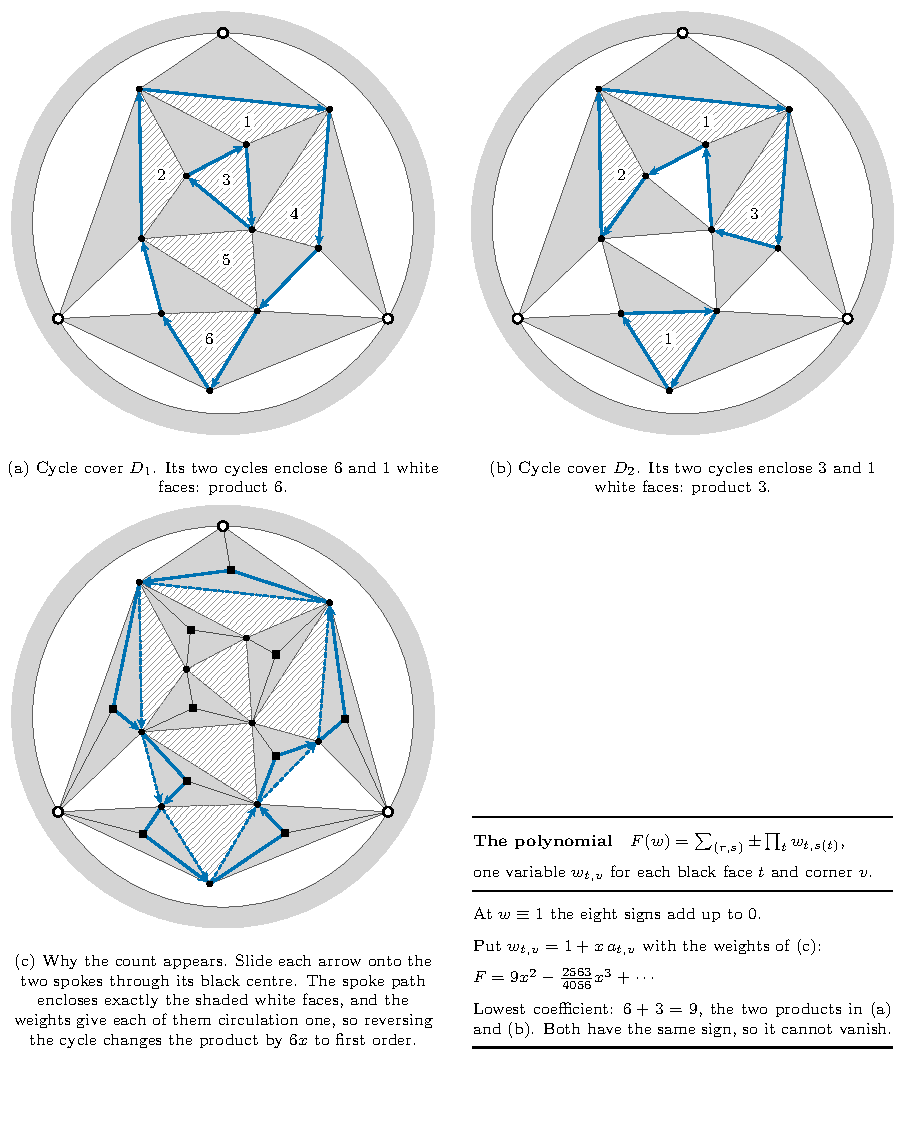
\includegraphics{figs/05-polynomial.pdf}\par}
\vfill\vfill Replace the exponential by a polynomial. Each pair contributes plus or minus a product of variables, one for each black face, picked by $s$. Cyclic states still cancel, because the two cancelling pairs pick the same variables. With every variable equal to one the polynomial is zero, since the signs balance. Move every variable a little in the direction of the spoke weights. Each cycle of $D$ then contributes the number of white faces inside it, and the lowest coefficient is a sum of positive products, here $6+3=9$. This version has integer coefficients and no analysis. The geometric input is unchanged, since positivity still comes from white faces inside disks.\par\smallskip \textbf{Status.} Proved in this project and checked by a second model. Not read by a human. The coefficients are computed here.\par\vfill
{\small\textbf{See also}\quad 4 (exponential sum), 3 (disk identity), 7 (heights).\par}
\clearpage\hypertarget{r6}{}\routetitle{6}{Cancellation as a pairing of objects}{main chain}
\vfill{\centering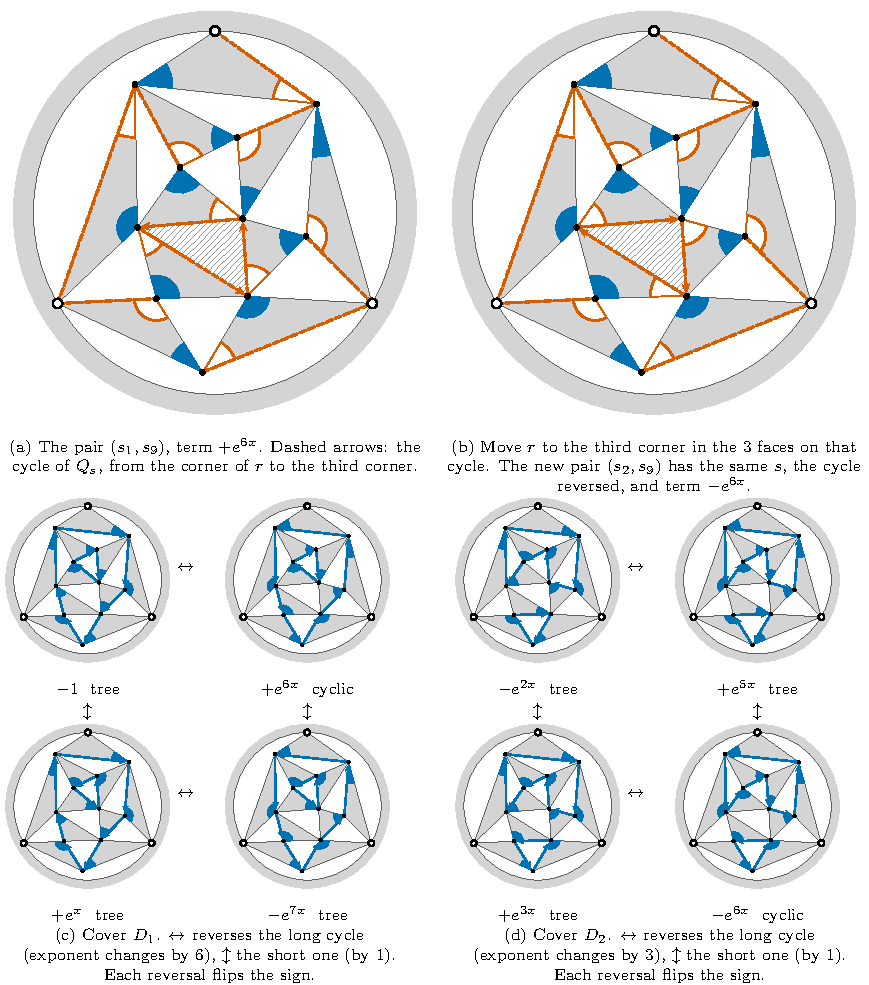
\includegraphics{figs/06-involutions.pdf}\par}
\vfill\vfill Li's note replaces the sum by two pairings. The first keeps $s$ fixed. If $Q_s$ has a cycle, move $r$ to the third corner on every face of that cycle, as in (a) and (b). The result is again a pair, with the opposite sign and the same weight, so the two cancel. With $k$ cycles the partners of $s$ form a cube with $2^k$ corners and the move pairs them all off. A state with a forest has one partner and survives. The second pairing must show that the survivors do not cancel each other. Reversing a cycle of $D$ flips the sign, as in (c) and (d), but it also changes the weight, so Li adds marks to make this a true pairing.\par\smallskip \textbf{Status.} Li's note, Definitions 13 to 23. The first pairing is computed here on all eight pairs. The atlas does not draw the marks, and the code for them was checked on the cube only.\par\vfill
{\small\textbf{See also}\quad 4 (exponential sum).\par}
\clearpage\hypertarget{r7}{}\routetitle{7}{The exponent is a volume}{main chain}
\vfill{\centering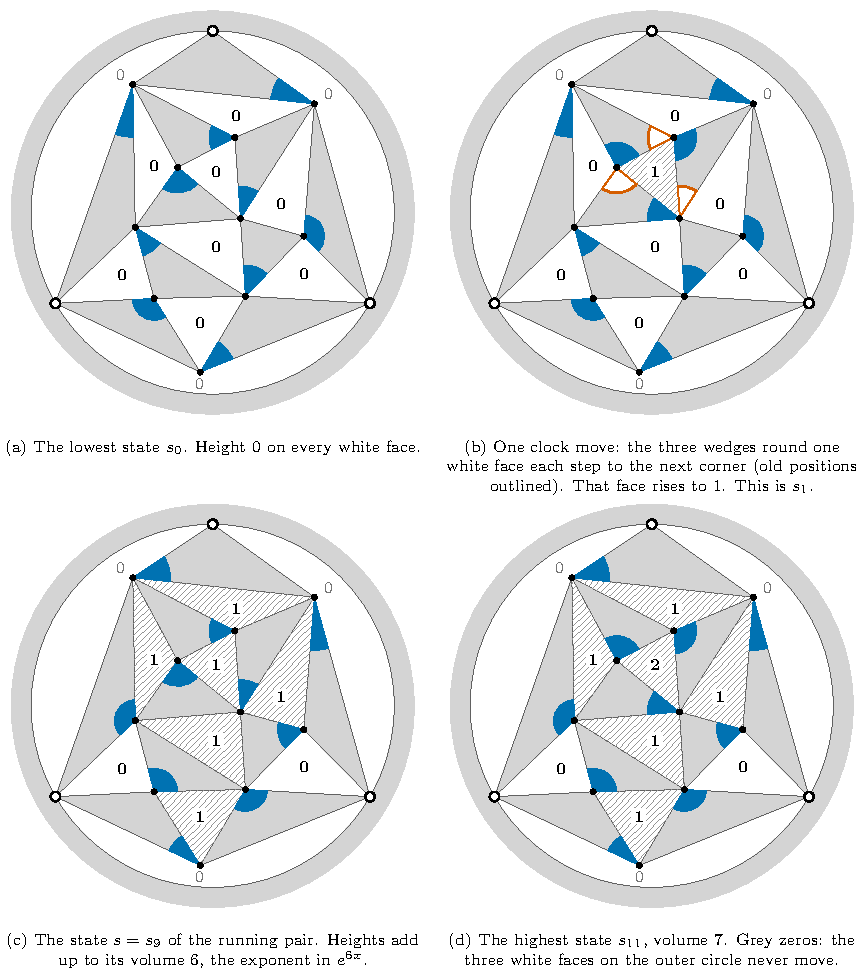
\includegraphics{figs/07-heights.pdf}\par}
\vfill\vfill The exponent has a picture. Fix the lowest state and compare any other state with it. The two differ along closed curves, and each white face gets the number of those curves that wind around it. That number is its height. One clock move turns the wedges around a white face and raises that face by one. The volume of a state is the sum of its heights, and the exponential sum weighs $s$ by $e$ to the volume times $x$. So the analytic weights count white faces under a surface, and reversing a cycle of $D$ changes the volume by the number of white faces inside the cycle.\par\smallskip \textbf{Status.} Proved in this project, with a corrected normalisation, and checked by a second model. Not read by a human. The heights of all twelve states are solved exactly here.\par\vfill
{\small\textbf{See also}\quad 4 (exponential sum), 5 (integer polynomial).\par}
\clearpage\hypertarget{r8}{}\routetitle{8}{From a forest state to the cycle}{main chain}
\vfill{\centering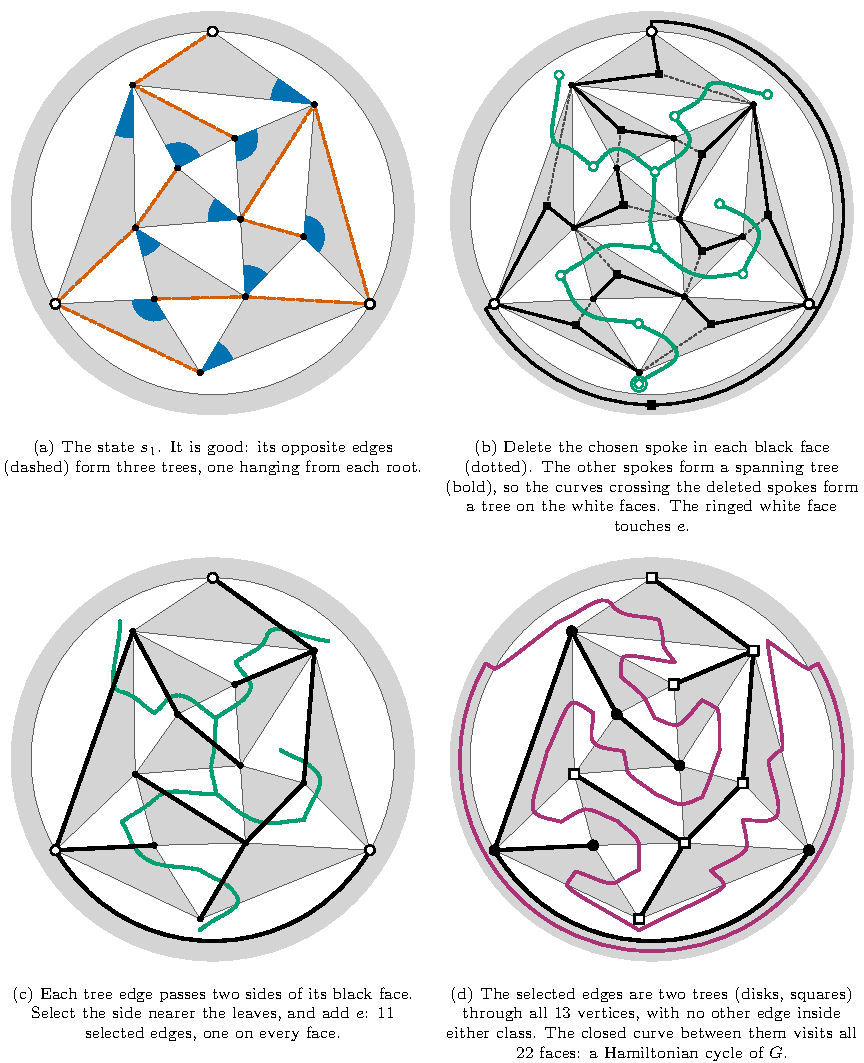
\includegraphics{figs/08-recovery.pdf}\par}
\vfill\vfill Once a state has a forest of opposite edges, the cycle follows with no further choices. Delete the chosen spoke in every black face. What remains of the spoke graph is a spanning tree, so the curves that cross the deleted spokes form a tree on the white faces. Root that tree at the white face next to the prescribed edge $e$. Each tree edge runs past two sides of one black face, and we select the side facing away from the root of the tree. The selected edges, with $e$, split the vertices of $T$ into two classes that each induce a tree. The boundary between the classes is one closed curve through every face. In $G$ it is a Hamiltonian cycle that avoids $e$.\par\smallskip \textbf{Status.} OpenAI paper, Section 6. Every object in the four panels is asserted by the checker and agrees with the independent laboratory code.\par\vfill
{\small\textbf{See also}\quad 1 (the chain), 9 (primal picture).\par}
\clearpage\hypertarget{r9}{}\routetitle{9}{The same proof inside the cubic graph}{main chain}
\vfill{\centering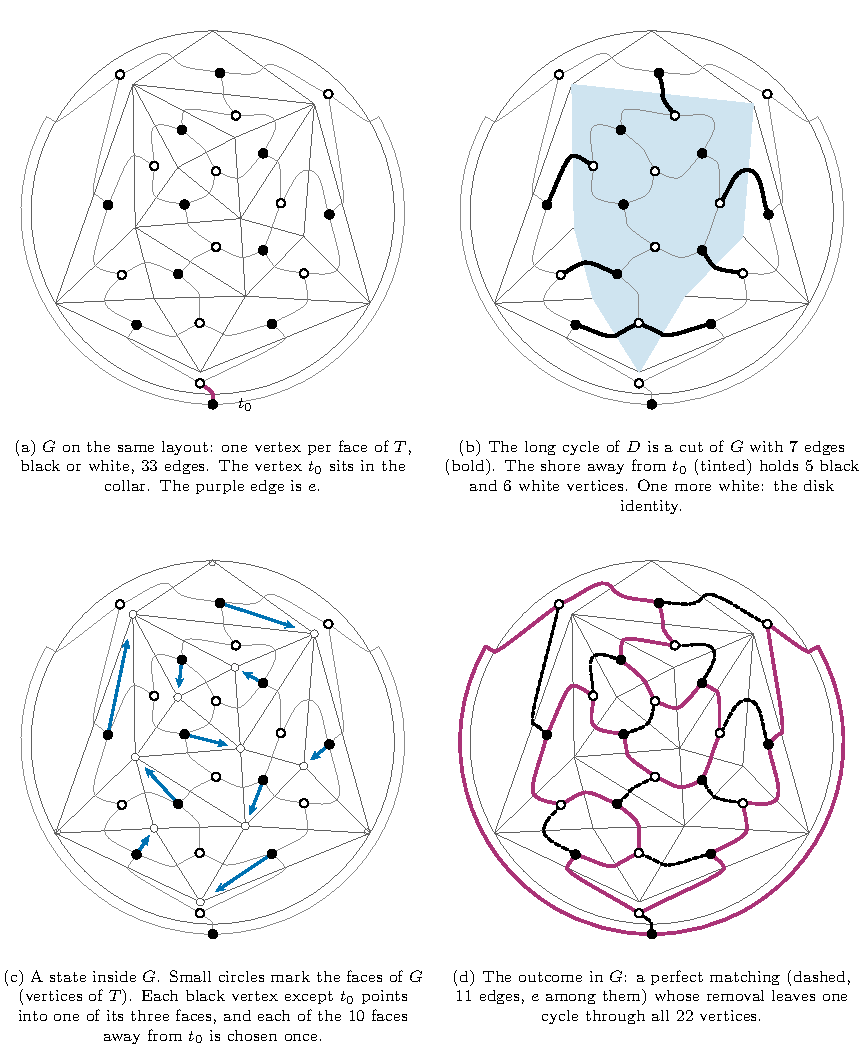
\includegraphics{figs/09-primal.pdf}\par}
\vfill\vfill Li's note and this project's primal write-up keep everything inside $G$. The vertices of $G$ are the faces of $T$, so black faces become black vertices and the vertices of $T$ become the faces of $G$. A state lets each black vertex choose one of its three faces. A cycle of $D$ becomes an edge cut, and its disk becomes the shore of that cut away from the root vertex. The disk identity says the shore has one more white vertex than black. The outcome also needs no duality. Removing a perfect matching that contains $e$ leaves a single cycle. The proof gets no shorter. The gain is that the inside of a curve is now a shore of a cut, which a proof assistant can handle without a picture.\par\smallskip \textbf{Status.} The primal proof was written in this project and refereed by a second model. The Lean statement of it is unrefereed. Not read by a human.\par\vfill
{\small\textbf{See also}\quad 3 (disk identity), 8 (recovery).\par}
\clearpage\noindent{\Large\bfseries Sources}\par\vspace{1mm}\hrule\medskip
{\small Each row lists the papers, the project reports and the computation behind one page. Paths are relative to the repository root. The build script draws every figure from objects it computes and asserts, and it writes the certificates to computed.json next to the atlas. Where a row says a report is unrefereed, no second model has checked it. No human mathematician has read any page of this atlas.\par}\medskip
{\footnotesize\setlength{\tabcolsep}{3pt}\begin{longtable}{@{}r>{\raggedright\arraybackslash}p{3.6cm}>{\raggedright\arraybackslash}p{11.2cm}@{}}\toprule
& Page & Sources and computation\\\midrule\endhead
1 & The chain & \path{papers/OpenAI-Barnette.pdf}, Sections 3 to 7; \path{digestions/route-map/ROUTE-MAP.md}; computed by \path{digestions/atlas/build.py}\\[.6mm]
2 & Two states & \path{papers/OpenAI-Barnette.pdf}, Proposition 3.1, Section 7; \path{toolkit/check.py} (cut inequality for all subsets); computed by \path{digestions/atlas/build.py}\\[.6mm]
3 & Disk identity & \path{papers/OpenAI-Barnette.pdf}, Lemma 4.1; \path{research/2026-11-14_astra_referee-combinatorics/REWRITTEN-PROP-5-1.md}; \path{research/2026-11-14_opus_route-topology/TOPOLOGY.md}, Section 2; \path{research/2026-11-14_fable_referee-topology/REFEREE.md}, parts a and b; computed by \path{digestions/atlas/build.py}\\[.6mm]
4 & Exponential sum & \path{papers/OpenAI-Barnette.pdf}, Proposition 5.1, Lemmas 5.2 and 5.3; computed by \path{digestions/atlas/build.py} (lib.py: term, \path{group_data})\\[.6mm]
5 & Integer polynomial & \path{research/2026-11-14_fable_referee-determinants/SIGNIFICANCE.md}, Section 2; \path{papers/barnette_trees.pdf} (signed integer polynomial); computed by \path{digestions/atlas/build.py} (lib.py: Fpoly)\\[.6mm]
6 & Involutions & \path{papers/A-Note-On-Barnette.pdf}, Definitions 13 to 23, Appendix B; \path{workings/barnette_lab/barnette_lab/li.py}; \path{research/2026-11-14_fable_referee-topology/REFEREE.md}, part d (Morse reading); computed by \path{digestions/atlas/build.py}\\[.6mm]
7 & Heights & \path{research/2026-11-14_astra_referee-combinatorics/REFEREE.md}; \path{research/2026-11-14_fable_referee-topology/REPORT.md} (height as winding number); computed by \path{digestions/atlas/build.py} (lib.py: heights)\\[.6mm]
8 & Recovery & \path{papers/OpenAI-Barnette.pdf}, Section 6; \path{papers/barnette_trees.pdf} (recovery criterion); \path{toolkit/model.py} (recover); computed by \path{digestions/atlas/build.py}\\[.6mm]
9 & Primal picture & \path{papers/A-Note-On-Barnette.pdf}; \path{proofs/primal/}; \path{research/2026-11-14_astra_primal-proof/}; \path{research/2026-11-14_fable_referee-primal/}; \path{research/2026-11-14_opus_lean-formalisation/REPORT.md}; computed by \path{digestions/atlas/build.py}\\[.6mm]
\bottomrule\end{longtable}}
\end{document}
